\setAuthor{Kaur Aare Saar}
\setRound{lõppvoor}
\setYear{2021}
\setNumber{G 5}
\setDifficulty{5}
\setTopic{TODO}

\prob{Võimsus}
Juuresoleval skeemil on alguses lüliti avatud. Leidke takistitel eralduv koguvõimsus \\
\osa vahetult pärast lüliti sulgemist; \\
\osa pika aja möödudes pärast lüliti sulgemist.\\
Kõikide takistite takistus on $R$ ja patarei pinge on $V$.
\vspace{-4pt}
\begin{figure}[h]
  \centering
  \begin{minipage}[h]{0.44\textwidth}
    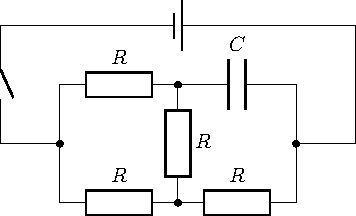
\includegraphics[width=\textwidth]{2021-v3g-05-yl.pdf}
  \end{minipage}
 \end{figure}
\vspace{-12pt}


\hint

\solu
Vahetult pärast lüliti sulgemist käitub kondensaator kui lühis. Järelikult on skeemi kogutakistus
\[
  R=\frac{1}{\frac 1R + \frac 2{3R}}=\frac 35 R
\]
Pärast pika aja möödumist käitub kondensaator kui avatud lüliti. Seega takistus on
\[
  R=R+\frac{1}{\frac 1R + \frac 1{2R}}=\frac 53 R
\]
Võimsused on seega vastavalt $P=\frac{5V^2}{3R}$ ja $P=\frac{3V^2}{5R}$.
\probend